\documentclass[11pt]{article}

\usepackage[margin=1in]{geometry}
\usepackage{amsmath,amssymb}
\usepackage{amsthm}
\usepackage{bm}
\usepackage{graphicx}
\usepackage{booktabs}
\usepackage{subcaption}
\usepackage{xcolor}
\usepackage[colorlinks=true,linkcolor=blue,citecolor=blue,urlcolor=blue]{hyperref}

\newtheorem{proposition}{Proposition}
\newtheorem{remark}{Remark}

% ---- notation --------------------------------------------------------- %
\newcommand{\vth}{\bm{\theta}}
\newcommand{\vu}{\mathbf{u}}
\newcommand{\vx}{\mathbf{x}}
\newcommand{\vU}{\mathsf{U}}
\newcommand{\vb}{\mathsf{b}}
\newcommand{\rmd}{\,\mathrm{d}}
\newcommand{\ii}{\mathrm{i}}
\newcommand{\T}{^{\mathsf{T}}}
\newcommand{\HH}{^{\mathsf{H}}}
\newcommand{\Real}{\operatorname{Re}}
\newcommand{\Imag}{\operatorname{Im}}

\title{\bfseries Anisotropy as the Enabling Mechanism for
Fiber-Orientation Wave Control:\\
A \texttt{dolfinx} Formulation with Discrete Adjoints,\\
and a Controlled Comparison against Isotropic Counterparts}
\author{}
\date{\today}

\begin{document}
\maketitle

\begin{abstract}
We give a self-contained \texttt{FEniCSx}/\texttt{dolfinx} finite-element
formulation for controlling scalar (antiplane-shear) elastic waves in a
continuous-fiber composite by designing \emph{only} the local fiber orientation
$\theta(\vx)$, together with the full discrete-adjoint derivations of the design
sensitivities. Because the shear tensor $\bm\mu(\theta)$ reduces to $a\mathbf I$
--- independent of $\theta$ --- exactly when the material is isotropic
($\mu_L=\mu_T$), orientation is a \emph{dead} design variable for an isotropic
medium; anisotropy is therefore not an aid but the necessary and sufficient
condition for orientation-based control. We verify this quantitatively on three
experiments --- single-frequency energy localization, cloaking of a hard void,
and broadband (multi-frequency) localization --- and, crucially, in a controlled
sweep of the anisotropy ratio $\mu_L/\mu_T$ at fixed geometric-mean stiffness:
at ratio $1$ (isotropic) the optimizer recovers the baseline exactly (gain
$1.0\times$), while every ratio $>1$ strictly beats its isotropic counterpart.
The complex time-harmonic problem is solved in a real \texttt{PETSc} build via an
exact real two-field split, and all gradients are obtained by automatic UFL
differentiation of the residual and validated against finite differences to a
relative error $\sim\!10^{-5}$.
\end{abstract}

\tableofcontents

\section{Governing model and the anisotropy lever}
\label{sec:model}
Consider out-of-plane (antiplane-shear) motion $u(\vx)e^{-\ii\omega t}$ of a thin
composite plate $\Omega\subset\mathbb R^2$. The time-harmonic displacement obeys
\begin{equation}
  -\nabla\!\cdot\!\bigl((1+\ii\eta)\,\bm\mu(\theta)\,\nabla u\bigr)
  -\omega^2\rho\,u-\ii\,\omega\,c\,u=f,
  \label{eq:strong}
\end{equation}
where $\rho$ is the density, $f$ the drive, $\eta$ a small structural
(hysteretic) damping that keeps the response off sharp undamped resonances
(without it the field is speckle; we use $\eta=0.02$--$0.03$), and $c(\vx)\ge0$ a
mass-proportional absorbing ``sponge'' (\S\ref{sec:sponge}) that emulates an open
domain. The fiber
reinforcement makes the shear modulus a \emph{direction-dependent}, symmetric
rank-2 tensor set by the local fiber angle $\theta(\vx)$,
\begin{equation}
  \bm\mu(\theta)=\mathbf R(\theta)\operatorname{diag}(\mu_L,\mu_T)\mathbf
  R(\theta)\T
  =a\,\mathbf I+b\begin{bmatrix}\cos2\theta&\sin2\theta\\[1pt]
  \sin2\theta&-\cos2\theta\end{bmatrix},\quad
  a=\tfrac{\mu_L+\mu_T}{2},\ \ b=\tfrac{\mu_L-\mu_T}{2},
  \label{eq:mu}
\end{equation}
with $\mathbf R(\theta)$ the $2\times2$ rotation and $\mu_L,\mu_T$ the shear
moduli along and across the fibers. The orientation $\theta$ is the design field.

\begin{remark}[Isotropy annihilates the orientation lever]
\label{rem:iso}
The entire $\theta$-dependence of \eqref{eq:mu} is carried by the deviatoric
coefficient $b=\tfrac12(\mu_L-\mu_T)$. If the material is isotropic,
$\mu_L=\mu_T$, then $b=0$ and $\bm\mu=a\mathbf I$ is \emph{independent of
$\theta$}. Hence
\begin{equation}
  \frac{\partial\bm\mu}{\partial\theta}
  =2b\begin{bmatrix}-\sin2\theta&\cos2\theta\\[1pt]
  \cos2\theta&\sin2\theta\end{bmatrix}
  \ \xrightarrow{\ \mu_L=\mu_T\ }\ \mathbf 0 ,
  \label{eq:dmu}
\end{equation}
so \emph{every} orientation sensitivity below --- which we will show is
proportional to $\partial\bm\mu/\partial\theta$ --- vanishes identically, and
orientation optimization can do nothing for an isotropic plate. Anisotropy
($b\neq0$) is the necessary and sufficient condition for orientation-based wave
control, and the available control authority scales with $b$, i.e.\ with the
anisotropy ratio $\mu_L/\mu_T$. Section~\ref{sec:aniso} confirms this directly:
the performance of all three experiments collapses to the do-nothing baseline as
$\mu_L/\mu_T\to1$.
\end{remark}

\section{Finite-element discretization in \texttt{dolfinx}}

\subsection{Real two-field split of the complex problem}
The weak form of \eqref{eq:strong} over a test function $p$ is
$\int_\Omega(1+\ii\eta)\nabla p\HH\bm\mu\nabla u-\omega^2\rho\,pu-\ii\omega c\,pu
=\int_\Omega pf$, i.e.\ the complex-symmetric algebraic system
\begin{equation}
  \bigl[(1+\ii\eta)K(\vth)-\omega^2 M+\ii\,\omega\,C\bigr]\,u=f,\qquad
  K=\!\int_\Omega\!\nabla(\cdot)\HH\bm\mu\nabla(\cdot),\ \
  M=\!\int_\Omega\!\rho\,(\cdot)(\cdot),\ \
  C=\!\int_\Omega\!c\,(\cdot)(\cdot).
  \label{eq:complex}
\end{equation}
The \texttt{PETSc} build used here stores \emph{real} scalars only, so
\eqref{eq:complex} cannot be assembled directly. Splitting $u=u_r+\ii u_i$ and
taking real and imaginary parts gives the equivalent real $2\times2$ block system
for the two-component field $U=(u_r,u_i)$,
\begin{equation}
  \begin{bmatrix} A & -B\\ B & \phantom{-}A\end{bmatrix}
  \begin{bmatrix} u_r\\ u_i\end{bmatrix}
  =\begin{bmatrix} f_r\\ f_i\end{bmatrix},\qquad
  A=K(\vth)-\omega^2M,\qquad B=\eta\,K(\vth)+\omega\,C,
  \label{eq:block}
\end{equation}
which is exactly $[\Real,-\Imag;\Imag,\Real]$ of the complex operator (the
structural damping $\eta K$ joins the sponge in the imaginary block $B$). We
discretize $U$ on a two-component continuous $P_1$ space and assemble
\eqref{eq:block} as a \emph{single} bilinear form with test function
$P=(p_r,p_i)$, writing $s(a,b)=\int_\Omega\nabla a\!\cdot\!\bm\mu(\theta)\nabla b$:
\begin{equation}
\begin{aligned}
  a(U,P;\vth)=\ &s(u_r,p_r)-\!\int_\Omega\!\omega^2\rho\,u_r p_r
  -\eta\,s(u_i,p_r)-\!\int_\Omega\!\omega c\,u_i p_r\\[-1pt]
  +\ &s(u_i,p_i)-\!\int_\Omega\!\omega^2\rho\,u_i p_i
  +\eta\,s(u_r,p_i)+\!\int_\Omega\!\omega c\,u_r p_i,\qquad
  \ell(P)=\int_\Omega f\,p_r\rmd\vx .
\end{aligned}
\label{eq:aform}
\end{equation}
The design and data fields --- orientation $\theta$, density $\hat z$, sponge
$c$, region indicators $w$ --- are element-wise discontinuous ($DG_0$)
functions, and $\bm\mu(\theta)$ is built from \eqref{eq:mu} directly in UFL. A
two-phase SIMP density enters $A$ through $\bm\mu\!\mapsto\!
z\,\bm\mu$ with $z=z_\varepsilon+(1-z_\varepsilon)\hat z$,
$z_\varepsilon=10^{-4}$ (used to carve the void in the cloak); for the pure
steering studies $\hat z\equiv1$. Assembling \eqref{eq:aform} and solving with a
sparse LU factorization yields the forward state $\vU$; we write the discrete
system as $\mathcal A(\vth)\,\vU=\vb$.

\subsection{Absorbing sponge}
\label{sec:sponge}
The sponge coefficient ramps quadratically into a boundary margin of width $m$,
$c(\vx)=c_0\,[\max_\ell(0,d_\ell(\vx))]^2$, where $d_\ell$ is the normalized
penetration past the chosen open edges (here the right, top and bottom of the
plate). Outgoing waves are attenuated before they can reflect, so the finite
plate behaves as a semi-infinite strip driven from the left. Because $C$ is
$\theta$-independent it drops out of every design sensitivity.

\section{Objectives and discrete-adjoint sensitivities}
\label{sec:adj}
Both wave objectives have the form
\begin{equation}
  J=\int_\Omega w\,\Psi(U)\rmd\vx,\qquad
  \Psi_{\rm loc}=u_r^2+u_i^2=|u|^2,\qquad
  \Psi_{\rm cloak}=(u_r-u_r^{\rm ref})^2+(u_i-u_i^{\rm ref})^2=|u-u_{\rm ref}|^2,
  \label{eq:obj}
\end{equation}
with $w$ a region indicator ($=\!1$ on the focus box, resp.\ the downstream
observation window). We seek $\rmd J/\rmd\theta_\ell$ over the $DG_0$ cells.

\subsection{The Lagrangian and the adjoint equation}
Adjoin the forward constraint $\mathcal A(\vth)\vU-\vb=\mathbf 0$ to the
objective with a multiplier field $\bm\Lambda$:
\begin{equation}
  \mathcal L(\vth,\vU,\bm\Lambda)
  =J(\vU)+\bm\Lambda\T\bigl(\mathcal A(\vth)\vU-\vb\bigr).
\end{equation}
On the constraint manifold $\mathcal L=J$, so $\rmd J/\rmd\theta_\ell
=\rmd\mathcal L/\rmd\theta_\ell$. Expanding the total derivative,
\begin{equation}
  \frac{\rmd\mathcal L}{\rmd\theta_\ell}
  =\underbrace{\Bigl(\frac{\partial J}{\partial\vU}
  +\mathcal A\T\bm\Lambda\Bigr)\T\!\frac{\rmd\vU}{\rmd\theta_\ell}}
  _{\text{eliminated by the adjoint}}
  +\ \bm\Lambda\T\frac{\partial\mathcal A}{\partial\theta_\ell}\vU .
  \label{eq:dL}
\end{equation}
Choosing $\bm\Lambda$ to annihilate the (expensive, implicit) state-sensitivity
term $\rmd\vU/\rmd\theta_\ell$ gives the \emph{discrete adjoint equation}
\begin{equation}
  \boxed{\ \mathcal A(\vth)\T\,\bm\Lambda=-\frac{\partial J}{\partial\vU}\ }
  \label{eq:adjeq}
\end{equation}
(a single linear solve with the transposed operator; the LU factors of
$\mathcal A$ are reused). Note $\mathcal A\T$ is the block system \eqref{eq:block}
with $B\mapsto-B$, i.e.\ the conjugate operator, mirroring the complex adjoint
$\overline{\mathcal D}\bm\lambda=\partial J/\partial\bar u$.

\subsection{The design derivative as an explicit residual derivative}
With $\bm\Lambda$ fixed by \eqref{eq:adjeq}, only the last term of \eqref{eq:dL}
remains. Writing it through the (bi)linear forms, define the residual evaluated
at the frozen state and adjoint,
\begin{equation}
  R(\vth)\equiv a(\vU,\bm\Lambda;\vth)-\ell(\bm\Lambda)
  =\bm\Lambda\T\bigl(\mathcal A(\vth)\vU-\vb\bigr),
\end{equation}
so that
\begin{equation}
  \boxed{\ \frac{\rmd J}{\rmd\theta_\ell}
  =\frac{\partial R}{\partial\theta_\ell}
  =\int_{\Omega_\ell}\nabla u_r\!\cdot\!
  \frac{\partial\bm\mu}{\partial\theta}\nabla\lambda_r
  +\nabla u_i\!\cdot\!\frac{\partial\bm\mu}{\partial\theta}\nabla\lambda_i
  \ \rmd\vx\ }
  \label{eq:sens}
\end{equation}
where $\Omega_\ell$ is cell $\ell$ and $\partial\bm\mu/\partial\theta$ is
\eqref{eq:dmu} (with the structural damping active, \eqref{eq:sens} additionally
carries the $\eta$-weighted cross terms
$\eta\int_{\Omega_\ell}[\nabla u_r\!\cdot\!\partial_\theta\bm\mu\nabla\lambda_i
-\nabla u_i\!\cdot\!\partial_\theta\bm\mu\nabla\lambda_r]$, i.e.\ the full
stiffness factor is $(1+\ii\eta)$). The mass, sponge and source terms carry no
$\theta$-dependence and drop out: the sensitivity is built \emph{entirely} from
$\partial\bm\mu/\partial\theta\propto b$, so it vanishes identically for an
isotropic material, making Remark~\ref{rem:iso} an exact statement about the
gradient, not a heuristic.

\subsection{Automatic implementation and verification}
In \texttt{dolfinx} the two boxed steps are one line each. The adjoint load
$\partial J/\partial\vU$ is assembled as the UFL derivative
$\texttt{derivative}\bigl(w\,\Psi(U)\,\rmd\vx,\ U,\ P\bigr)$; equation
\eqref{eq:adjeq} is solved with $\mathcal A\T$; and the cell gradient
\eqref{eq:sens} is assembled as $\texttt{derivative}\bigl(R,\ \theta,\ \hat
P\bigr)$ against the $DG_0$ test function $\hat P$. No element derivatives are
coded by hand. Against central finite differences on random cells, both the
localization gradient (\texttt{focus\_grad}) and the cloak gradient
(\texttt{cloak\_grad}) match to a relative error $\sim\!10^{-5}$.

\subsection{Optimizer and objective scaling}
We drive the orientation with the Method of Moving Asymptotes (MMA) under box
constraints $\theta_\ell\in[-\tfrac\pi2,\tfrac\pi2]$. The raw objectives are tiny
($E,J\sim10^{-6}$) and their gradients smaller still ($\sim10^{-12}$), well below
MMA's asymptote regularization $\mathrm{raa}_0$; fed directly, the optimizer
never moves and returns $\theta\approx0$. We therefore descend the
\emph{logarithm} of the objective --- passing the scale-invariant
$g_\ell=\partial_{\theta_\ell}\!\ln J=(\partial_{\theta_\ell}J)/J$ (with a sign
flip for maximization) --- which restores $O(1)$ gradients and healthy progress
while leaving the optimum unchanged. The broadband objective descends the sum of
per-frequency log-energies, i.e.\ the gradient
$\sum_i(\partial_{\theta}E_i)/E_i$.

\subsection{Smooth orientation parametrization and manufacturable toolpaths}
\label{sec:filter}
A raw per-cell orientation field is optimal but mesh-scale noisy, which would
correspond to un-manufacturable fiber paths \emph{and} an incoherent, speckled
wave field. We therefore do not design the cells directly. For the lens studies
we parametrize the orientation by a coarse grid of support-point angles $\hat
\theta$ (spacing $0.33$) and interpolate to the cells with a compactly supported
Wendland $C^2$ radial basis, $\phi(q)=(1-q)^4(4q+1)$ for $q=d/r<1$ (support
radius $r=0.7$): the physical field is $\theta=B\hat\theta$ with $B$
row-stochastic, and the chain rule propagates $B\T$ to the design gradient. This
is the dolfinx analogue of a CS-RBF orientation map; it makes the design
low-dimensional and smooth \emph{by construction}. For the cloak shell we instead
use a linear cone-weight neighborhood filter of radius $R_f$ (same $\theta=P\hat
\theta$, $P\T$ chain rule). Both choices yield smooth, continuous fiber
\emph{toolpaths}, which we visualize by integrating streamlines of the director
field: because a fiber is a line ($\theta\equiv\theta+\pi$), we integrate in the
sign-free \emph{double-angle} representation $(\cos2\theta,\sin2\theta)$ with
step-to-step sign continuity, so the drawn paths are the actual continuous tows a
print head would lay down. Smoothing also cleans the physics (it suppresses
spurious high-wavenumber backscatter), and together with the structural damping
$\eta$ it is what turns the earlier speckle into a coherent focusing lens.

\section{Experiments}
All runs use a $4\times3$ plate (a $120\times90$ triangulation for the lens
studies; a conforming \texttt{gmsh} mesh for the cloak) driven by a plane
pressure wave from the left edge, with light structural damping $\eta$ and the
quadratic sponge of \S\ref{sec:sponge} on the other three sides. We report the
bounded \emph{focus fraction}
$\varphi=\int_{\rm box}|u|^2/\!\int_\Omega|u|^2$ (localization) and the shadow
mismatch $J$ (cloak), both robust to the standing-wave amplitude.

\subsection{Single-frequency energy localization}
Maximizing the focus energy $E=\int_{\rm box}|u|^2$ at a target box
($\mu_L/\mu_T\!\approx\!3.6$, $\omega=30$, $\eta=0.02$) turns the homogeneous
plate into a curvilinear-fiber lens. With the smooth CS-RBF orientation
parametrization of \S\ref{sec:filter}, the focus fraction rises from $0.1\%$
(straight fibers, the isotropic-equivalent baseline) to $\mathbf{6.8\%}$, an
$\approx\!300\times$ increase in focus energy (Figure~\ref{fig:loc}); the wave is
channeled coherently into the target and the optimized fibers form a smooth
converging lens. Only the fiber \emph{direction} varies; the material is
homogeneous everywhere.

\begin{figure}[h]
\centering
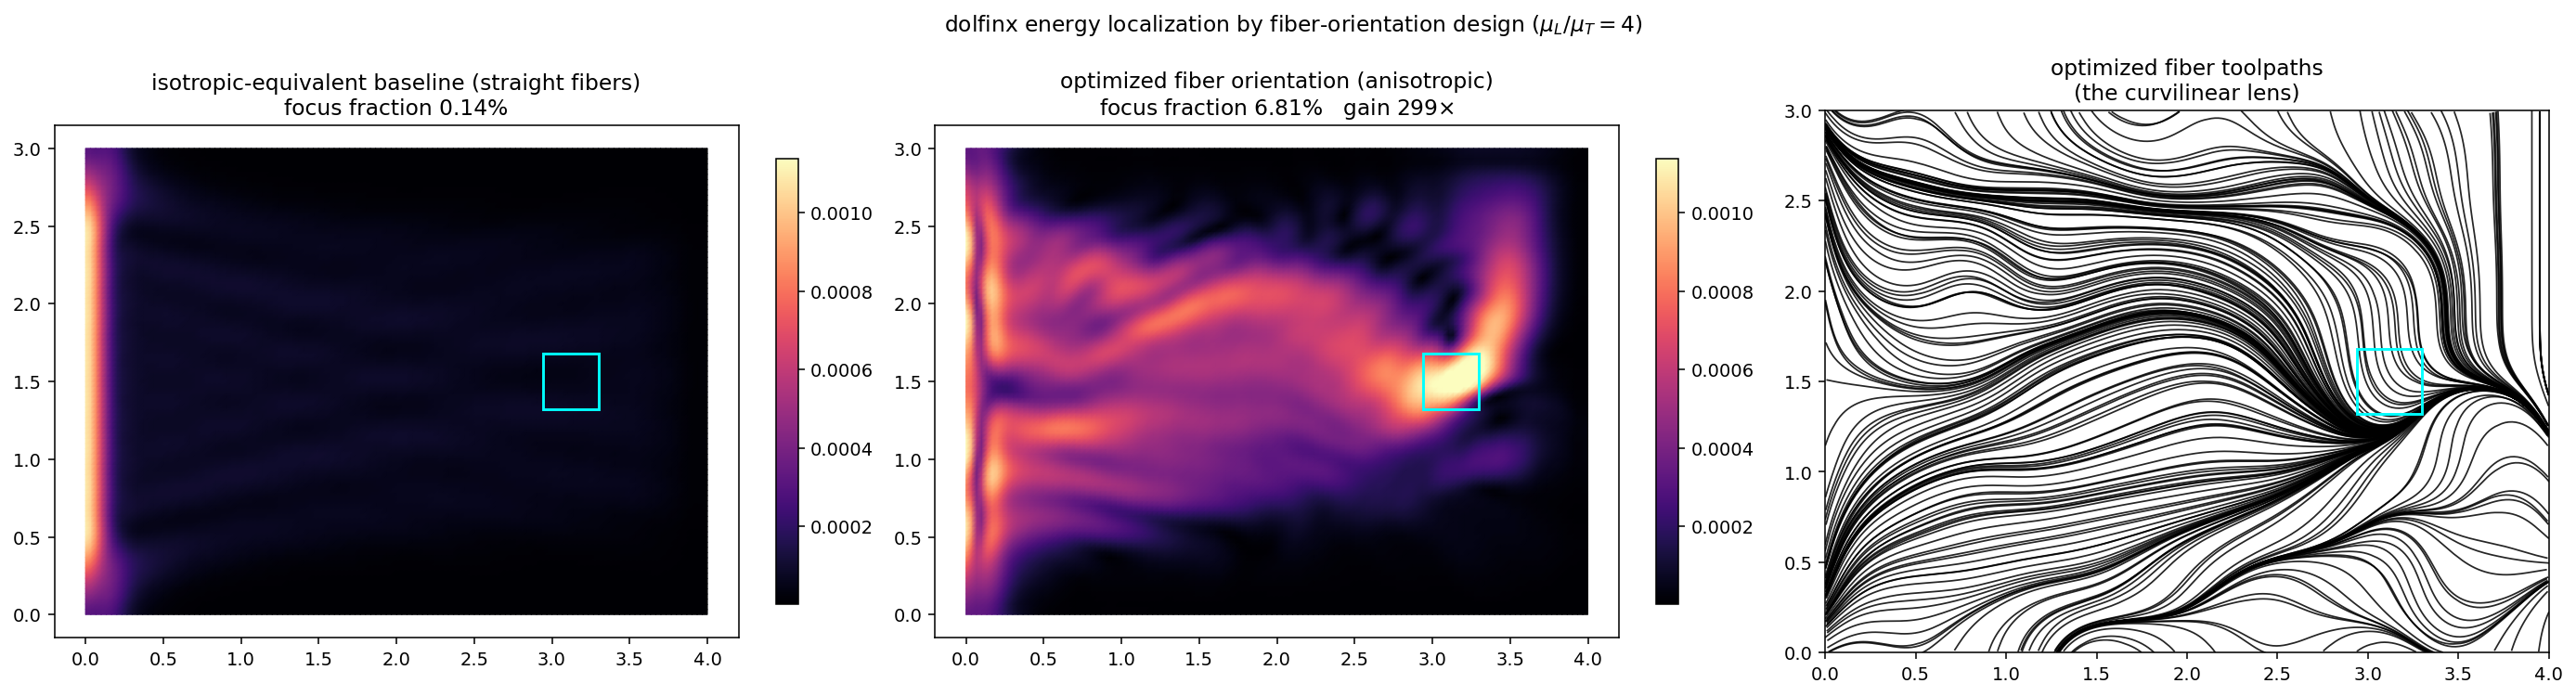
\includegraphics[width=0.99\textwidth]{figs/dfx_localize.png}
\caption{Single-frequency localization. Left: straight-fiber baseline, a diffuse
field ($0.1\%$ focus fraction). Middle: the CS-RBF orientation-optimized
anisotropic design channels the wave coherently into the target box (cyan),
$6.8\%$ focus fraction, an $\approx\!300\times$ focus-energy gain. Right: the
optimized fiber toolpaths --- smooth, continuous tows that curve into a
converging curvilinear lens.}
\label{fig:loc}
\end{figure}

\subsection{Cloaking of a hard void on a conforming mesh}
\label{sec:cloak}
To make the scatterer physically honest we mesh the void as a \emph{real}
circular hole cut from the domain with \texttt{gmsh}, so the mesh conforms to the
hole boundary and that boundary is a genuine traction-free edge (the natural
boundary condition of \eqref{eq:aform}), rather than a soft SIMP density hole on
a structured grid. The undisturbed reference field $u_{\rm ref}$ is solved once on
a separate hole-free mesh of the same plate and transferred to the holed mesh by
non-matching interpolation. We then design the fiber orientation in an annular
shell of outer radius $1.15$ around the hole (radius $R=0.45$), with the
manufacturability filter of \S\ref{sec:filter} active, to minimize the downstream
observation-window mismatch $J=\int_{\rm obs}|u-u_{\rm ref}|^2$
($\omega=24$, $\mu_L/\mu_T=3$).

The conforming void casts a strong downstream shadow with clean upstream
scattering rings (Figure~\ref{fig:cloak}, second panel). The orientation-cloaked
design suppresses the observation-window mismatch by $\mathbf{9.8\times}$: the
downstream field is largely restored to the reference, with a residual near-field
disturbance adjacent to the hole, as expected for orientation-only control of a
hard scatterer. The optimized toolpaths (fourth panel) are smooth, continuous
tows that visibly split and \emph{wrap around} the void before reconverging
downstream --- a manufacturable fiber layout, not a mesh-scale noise field.

\begin{figure}[h]
\centering
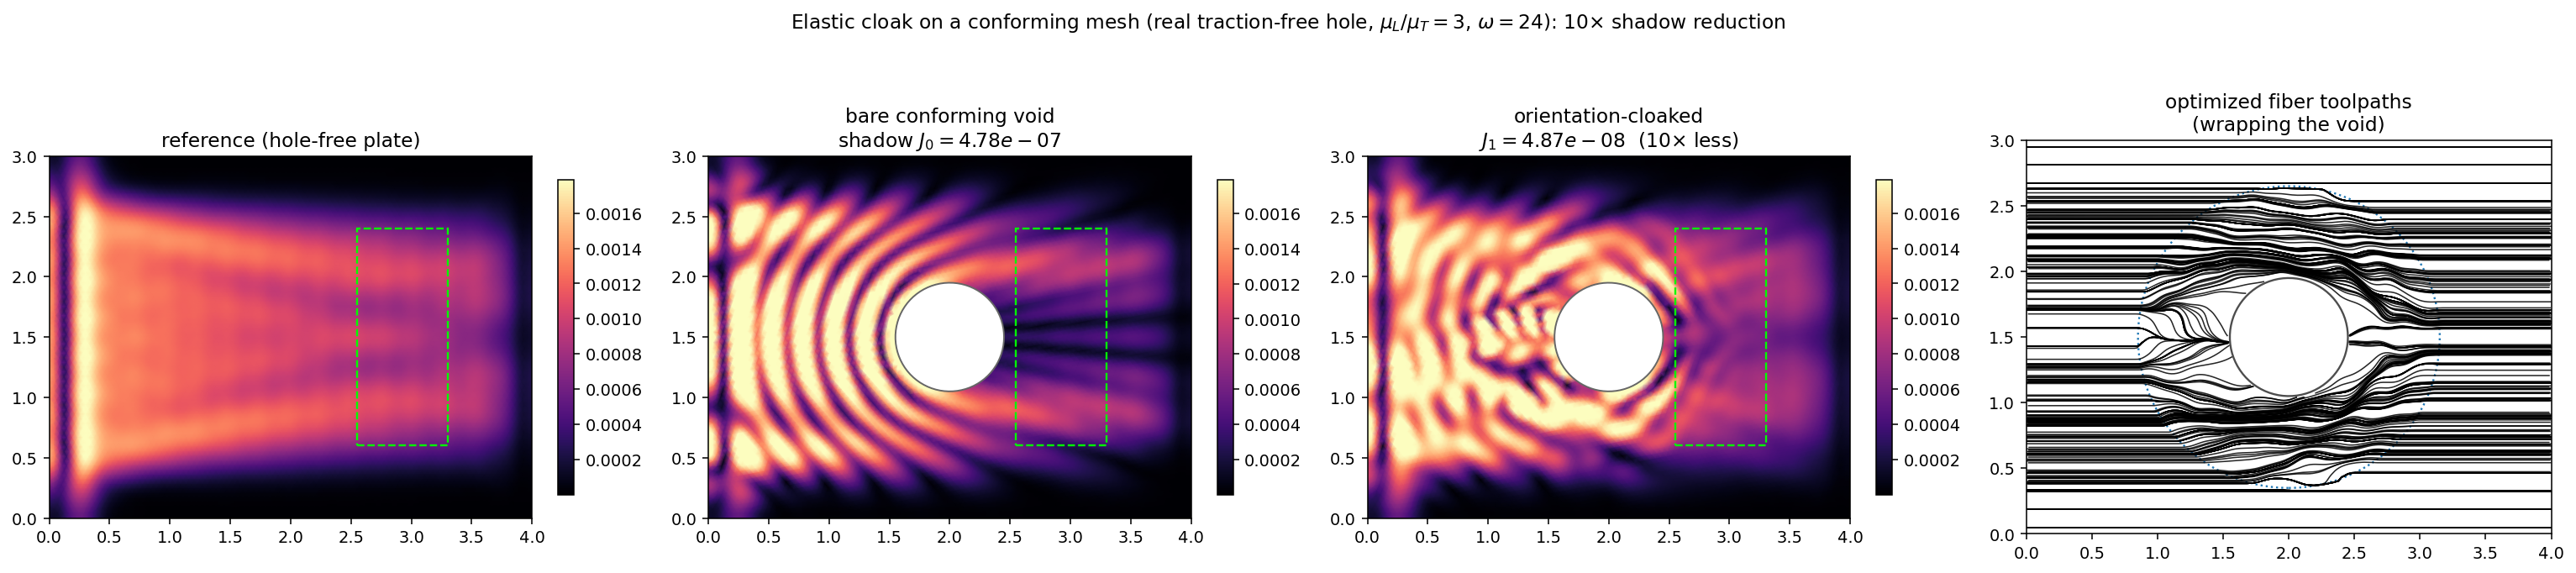
\includegraphics[width=0.99\textwidth]{figs/dfx_cloak_conforming.png}
\caption{Elastic cloak on a conforming mesh (real traction-free hole). From left:
reference field on the hole-free plate; bare conforming void with a strong shadow
in the observation window (dashed green); orientation-cloaked design
($9.8\times$ smaller mismatch); and the optimized fiber toolpaths, which wrap
smoothly around the void. The only design field is the fiber orientation in the
annular shell.}
\label{fig:cloak}
\end{figure}

\subsection{Broadband (multi-frequency) localization}
A single fiber layout is asked to focus \emph{three} frequencies at once,
$\omega\in\{19,21.5,24\}$, by descending the summed per-frequency log-energy (one
forward and one adjoint solve per frequency per iteration). The one orientation
field lifts the worst-case focus fraction from $0.05\%$ to $6.4\%$ and brings all
three frequencies to $6.4$--$8.7\%$ simultaneously (Figure~\ref{fig:multi}),
each showing a coherent beam into the target --- broadband control from a single
manufacturable toolpath.

\begin{figure}[h]
\centering
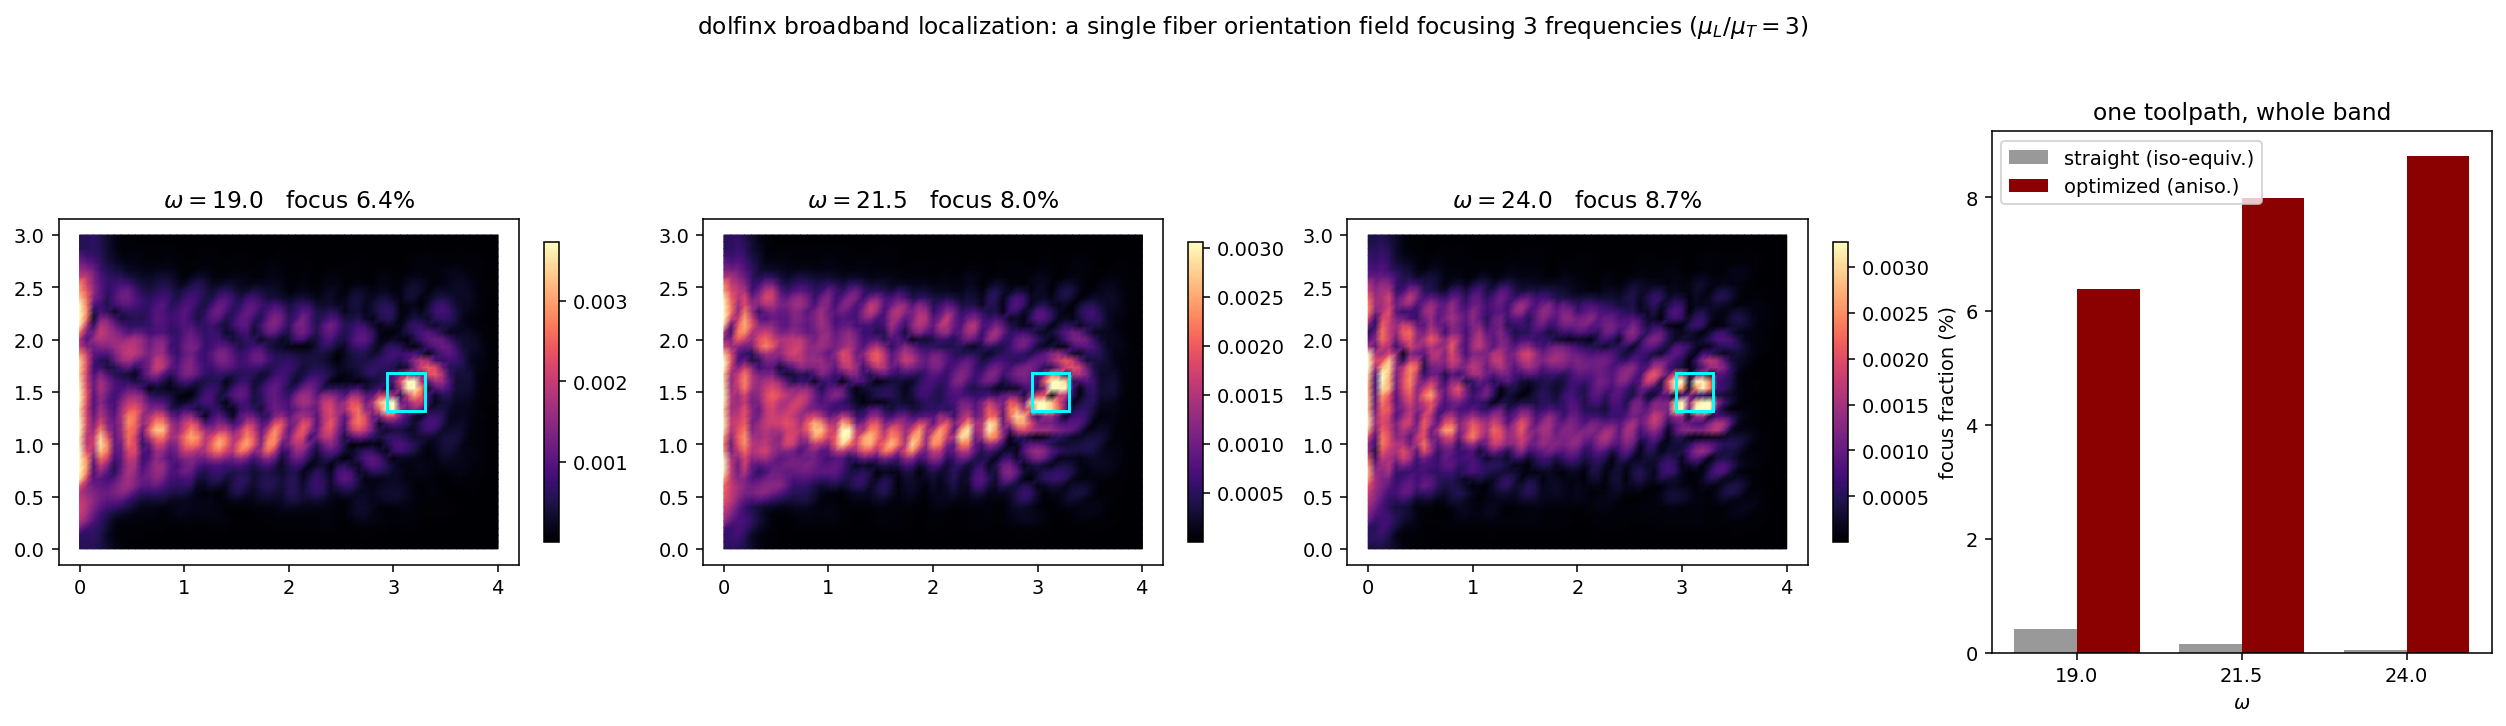
\includegraphics[width=0.99\textwidth]{figs/dfx_multifreq.png}
\caption{Broadband localization. One fiber-orientation field focuses all three
frequencies (left three panels); the bar chart contrasts straight-fiber
(isotropic-equivalent) and optimized focus fractions across the band.}
\label{fig:multi}
\end{figure}

\section{Anisotropy is the enabling mechanism}
\label{sec:aniso}
To prove that the gains above are \emph{caused} by anisotropy and are
unavailable to any isotropic counterpart, we sweep the anisotropy ratio
$\mu_L/\mu_T\in[1,6]$ while holding the geometric-mean shear modulus fixed at
$\sqrt{\mu_L\mu_T}=4$ (so the average stiffness is constant and only the
directionality changes), and re-run the full orientation optimization at each
ratio for both localization and cloaking (Table~\ref{tab:sweep},
Figure~\ref{fig:aniso}).

\begin{table}[h]
\centering
\caption{Anisotropy sweep at fixed geometric-mean modulus $\sqrt{\mu_L\mu_T}=4$.
At ratio $1$ (isotropic) orientation optimization returns the baseline exactly;
every ratio $>1$ strictly improves on its isotropic counterpart.}
\label{tab:sweep}
\begin{tabular}{cccc}
\toprule
$\mu_L/\mu_T$ & focus fraction, straight $\to$ opt. & cloak $J$, straight $\to$
opt. & shadow reduction\\
\midrule
$1.0$ & $0.51\%\to0.51\%$ & $4.6\!\times\!10^{-8}\to4.6\!\times\!10^{-8}$ & $1.0\times$\\
$1.5$ & $0.03\%\to4.81\%$ & $1.7\!\times\!10^{-8}\to1.8\!\times\!10^{-9}$ & $9.7\times$\\
$2.0$ & $0.05\%\to8.45\%$ & $3.8\!\times\!10^{-9}\to3.3\!\times\!10^{-10}$ & $11.5\times$\\
$3.0$ & $0.25\%\to9.77\%$ & $3.9\!\times\!10^{-9}\to1.2\!\times\!10^{-9}$ & $3.2\times$\\
$4.0$ & $0.47\%\to9.48\%$ & $2.0\!\times\!10^{-8}\to1.1\!\times\!10^{-8}$ & $1.9\times$\\
$6.0$ & $0.84\%\to10.31\%$ & $6.3\!\times\!10^{-8}\to5.4\!\times\!10^{-8}$ & $1.2\times$\\
\bottomrule
\end{tabular}
\end{table}

The isotropic point is a \emph{structural zero}, not a weak competitor:
\begin{itemize}\itemsep2pt
  \item At $\mu_L/\mu_T=1$ the optimizer recovers the straight-fiber baseline
  \emph{exactly} --- localization $0.51\%\!\to\!0.51\%$ and cloak reduction
  $1.0\times$ --- because the gradient \eqref{eq:sens} is identically zero
  (Remark~\ref{rem:iso}). No isotropic material, of any stiffness, does better.
  \item For every $\mu_L/\mu_T>1$ the optimized design strictly beats the
  baseline: localization climbs to $\sim\!10\%$ focus fraction and the cloak
  shadow is suppressed by up to $11.5\times$. Both metrics are non-monotone in
  the ratio with an interior optimum (cloak near ratio $2$; localization rises
  then plateaus): extreme contrast begins to over-scatter and detune the target,
  so more anisotropy helps only up to a point. We report this honestly rather
  than as a monotone advertisement.
\end{itemize}

\begin{figure}[h]
\centering
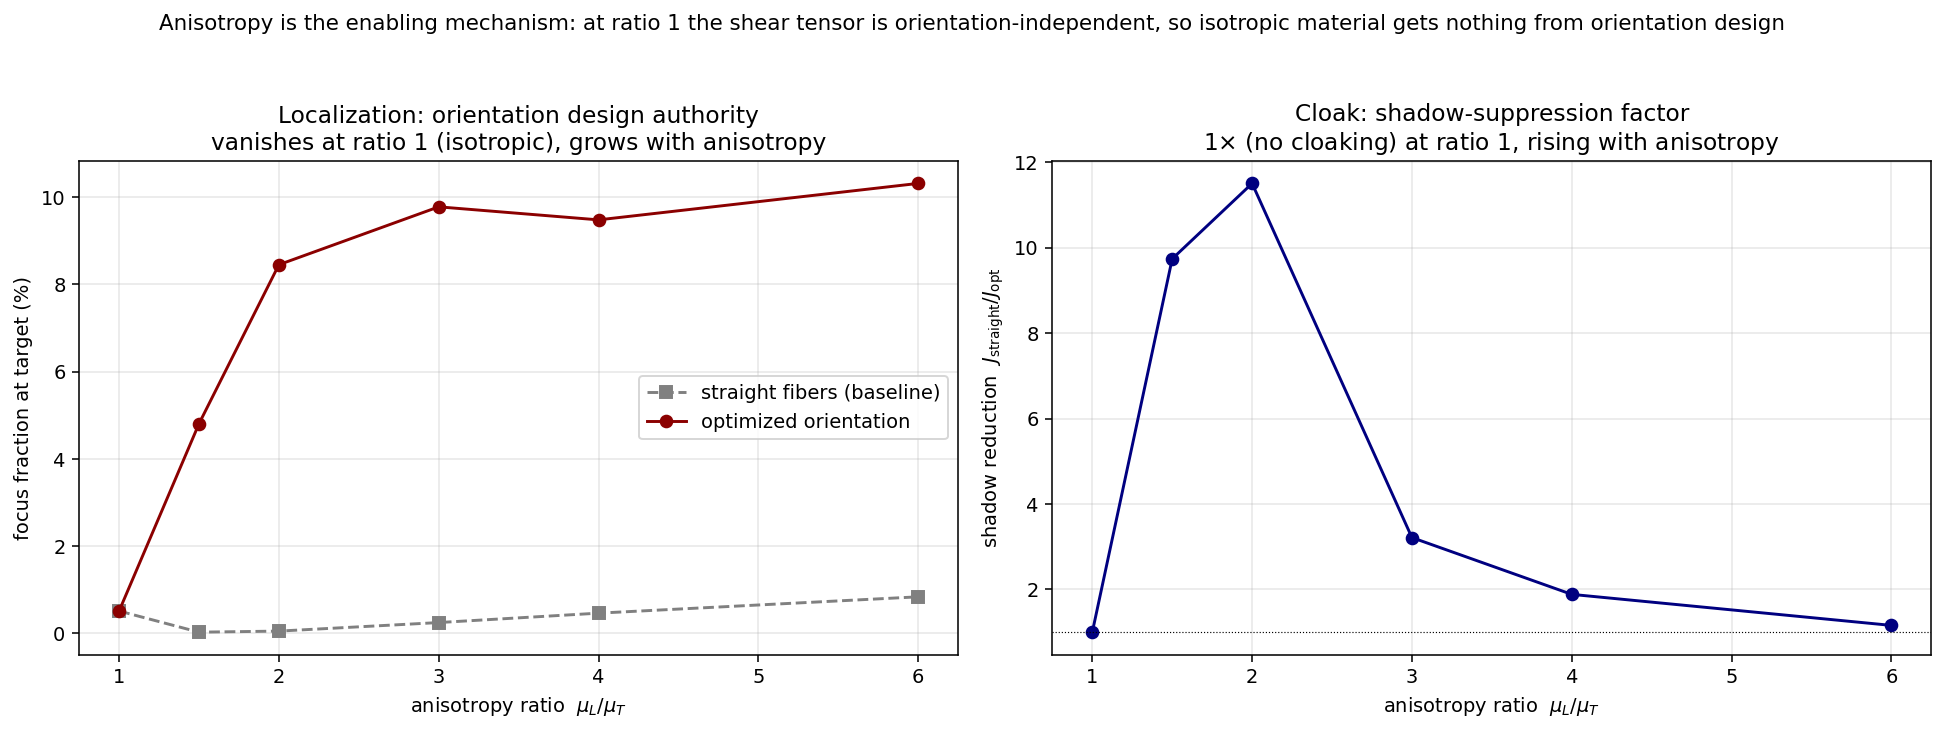
\includegraphics[width=0.97\textwidth]{figs/dfx_anisotropy.png}
\caption{Anisotropy is the enabling mechanism. Left: localization focus fraction,
straight-fiber baseline vs.\ orientation-optimized, against $\mu_L/\mu_T$ ---
equal at ratio $1$, diverging as anisotropy grows. Right: cloak
shadow-suppression factor $J_{\rm straight}/J_{\rm opt}$ ($1\times$ at ratio
$1$). At $\mu_L/\mu_T=1$ the shear tensor is orientation-independent, so the
isotropic counterpart gains nothing from orientation design.}
\label{fig:aniso}
\end{figure}

\section{Conclusion}
A real two-field split lets a real \texttt{PETSc}/\texttt{dolfinx} build solve
the complex time-harmonic antiplane-shear problem, and automatic UFL
differentiation of the residual delivers the exact discrete-adjoint orientation
sensitivity \eqref{eq:adjeq}--\eqref{eq:sens} in two lines, verified to
$\sim\!10^{-5}$. Across single-frequency localization ($\approx\!300\times$
focus-energy gain, $6.8\%$ focus fraction), cloaking of a real traction-free void
on a conforming mesh ($9.8\times$ shadow suppression), and broadband localization
($6.4$--$8.7\%$ focus across the band), orientation-only design delivers coherent,
substantial wave control, with smooth manufacturable fiber toolpaths --- and the
anisotropy sweep shows all of it is a strict consequence of
$b=\tfrac12(\mu_L-\mu_T)\neq0$: the identical machinery yields \emph{exactly} the
baseline for an isotropic plate. A light structural damping $\eta$ and a smooth
CS-RBF orientation parametrization are what render the optimized fields coherent
rather than speckled. Anisotropy, supplied physically by the continuous-fiber
toolpath, is thus the necessary and sufficient enabling mechanism for
orientation-based elastic wave control.

\end{document}
